% Intended LaTeX compiler: pdflatex
\documentclass[10pt,a4paper,UTF8]{article}
\usepackage{zclorg}
\author{张朝龙}
\date{}
\title{线性映射}
\hypersetup{
 pdfauthor={张朝龙},
 pdftitle={线性映射},
 pdfkeywords={},
 pdfsubject={},
 pdfcreator={Emacs 25.0.50.1 (Org mode 9.0.5)}, 
 pdflang={English}}
\begin{document}

\maketitle
\tableofcontents
\titlepic{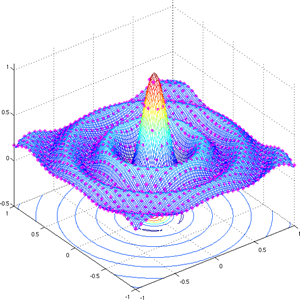
\includegraphics[scale=0.25]{../../img/sinc.PNG}}
\newpage



\section{向量空间的线性映射}
\label{sec:org500e39c}


\begin{definition}
从\(V\) 到\(W\)的线性映射是具有以下性质的函数\(T: V \rightarrow W\):

加性: 对所有\(u,v \in V\)都有 \(T(u+v) = T(u) + T(v)\)

齐次: 对所有的 \(\lambda \in \mathbf{F}\) 和\(v\in V\) 都有 \(T(\lambda v) = \lambda (Tv)\)
\end{definition}

从线性映射的定义可以看出,线性映射本质是函数,这个函数满足其次可加性。对于输入\(x\)可以拆解成\(x=u+v\)然后分别求出\(T(u),T(v)\),得\(T(x)=T(u)+T(v)\)。

我们把从\(V\)到\(W\)的所有线性映射的集合记为\(\mathcal{L}(V,W)\)。接下来我们看一些线性映射的例子:

\begin{instance}
零:除了其他用途,\(0\)也用来表示一个函数,他表示把某个空间的每个元素都映射为另一个空间的加法单位元。确切的说,\(0\in \mathcal{L}(V,W)\)。定义为\[0v = 0\]

等式左边的零表示从\(V\)到\(W\)的函数,右边的零表示\(W\)中的加法单位元。

恒等:恒等映射是某个向量空间上的函数,记为\(I\),它把每个元素都映射成自身,确切的说\(I\in \mathcal{L}(V,V)\),满足:\(Iv = v\)

微分:定义\(D\in \mathcal{L}(\mathcal{P}(\mathbf{R}),\mathcal{P}(\mathbf{R}))\),如下:\[Dp = p^{'}\]这个函数是线性的。

积分:定义\(T\in \mathcal{L}(\mathcal{P}(\mathcal{R}),\mathbf{R})\),如下:\[Tp = \int_{0}^{1} p(x)dx\]

乘以\(x^{2}\): 定义\(T\in \mathcal{L}(\mathcal{P}(\mathbf{R}),\mathcal{P}(\mathbf{R})\)

向后移位:\(T(x_{1},x_{2},x_{3},\ldots ) = (x_{2},x_{3},\ldots )\)

从\(\mathbf{R}^{3}\)到\(\mathbf{R}^{2}\) 定义 \(T\in \mathcal{L}(\mathbf{R}^{3}, \mathbf{R}^{2})\) :\[T(x,y,z) = (2x-y +3z,7x+5y-6z)\]
这个映射就有了矩阵的味道了:
\begin{equation}
\label{eq:1}
\begin{bmatrix}
u \\ v
\end{bmatrix}
=
\begin{bmatrix}
2 & -1 & 3 \\
7 & 5  & -6
\end{bmatrix}
\begin{bmatrix}
x \\ y \\ z
\end{bmatrix}
\end{equation}
\end{instance}

推而广之就有:
\begin{instance}
从\(\mathbf{F}^{n}\)到\(\mathbf{F}^{m}\),设\(m,n\)是正整数,\(A_{j,k}\in \mathbf{F},j = 1,\ldots ,m,k=1,\ldots ,n\),定义\(T\in \mathcal{L}(\mathbf{F}^{n}, \mathbf{F}^{m})\)为:
\begin{equation}
\label{eq:3}
T(x_{1},x_{2},\ldots ,x_{n}) = (A_{1,1}x_{1} + \ldots  + A_{1,n}x_{n}, \ldots , A_{m,1}x_{1} + \ldots + A_{m,n}x_{n})
\end{equation}
式\ref{eq:3}可以写成矩阵的形式为:
\begin{equation}
\label{eq:4}
\begin{bmatrix}
y_{1} \\ y_{2} \\ \vdots \\ y_{m}
\end{bmatrix}
=
\begin{bmatrix}
A_{1,1} & A_{1,2}  & \ldots & A_{1,n} \\
A_{2,1} & A_{2,2}  & \ldots & A_{2,n} \\
\vdots & \vdots  & \ddots & \vdots \\
A_{m,1} & A_{m,2}  & \ldots & A_{m,n} \\
\end{bmatrix}
\begin{bmatrix}
x_{1} \\ x_{2} \\ \vdots \\ x_{n}
\end{bmatrix}
\end{equation}
这里就有问题了,是不是所有的线性映射都可以写成矩阵的形式?如果是?为什么?如果不是,都有哪些线性映射可以写成矩阵的形式?那些不能写成矩阵的线性映射有什么特征?

关于这些问题的回答,在稍后的学习中会揭示。
\end{instance}

\begin{theorem}
设\(v_{1},\ldots ,v_{n}\)是\(V\)的基,\(w_{1},\ldots ,w_{n}\in W\),则存在唯一一个线性映射\(T:V\rightarrow W\) 使得对任意\(j=1,\ldots ,n\)都有:\[Tv_{j} = w_{j}\]
\end{theorem}
\begin{proof}
这个定理的证明需要从线性映射和基的定义出发。首先证明存在满足上述性质的线性映射\(T\),定义\(T:V\rightarrow W\)如下\[T(c_{1}v_{1}+ \ldots + c_{n}v_{n}) = c_{1}w_{1} + \ldots + c_{n}w_{n}\] 其中\(c_{1},\ldots ,c_{n}\in \mathbf{F}\),由于\(v_{1},\ldots ,v_{n}\)是\(V\)的基,所以上面的等式的确定义了从\(V\)到\(W\)的函数\(T\)。(因为\(V\)的每个元素都可以唯一的表示成\(c_{1}v_{1} +\ldots +c_{n}v_{n}\)的形式)。 接下来我们证明映射\(T\)是线性映射。

首先证明可加性,然后证明齐次性(因为比较简单,所以略去)。

接下来证明这个线性映射的唯一性,现在假设\(T\in \mathcal{L}(V,W)\)且\(Tv_{j} = w_{j},j = 1,\ldots ,n\)设\(c_{1},\ldots ,c_{n}\in \mathbf{F}\) 由于\(T\)的齐次性,有\(T(c_{j}v_{j}) = c_{j}w_{j},j = 1,\ldots ,n\)由于\(T\)的可加性有:
\[T(c_{1}v_{1} + \ldots + c_{n}v_{n}) = c_{1}w_{1} + \ldots + c_{n}w_{n}\]

所以\(T\)在\(span(v_{1},\ldots ,v_{n})\)上由上式唯一确定。由于\(v_{1},v_{2},\ldots ,v_{n}\)是\(V\)的基,则\(T\)在\(V\)上是唯一确定的。
\end{proof}

我们用\(\mathcal{L}(V,W)\)表示从\(V\)到\(W\)的线性映射的集合。我们可以定义 \(\mathcal{L}(V,W)\)上的加法和标量乘法。设\(S,T\in \mathcal{L}(V,W)\) ,\(\lambda \in \mathbf{F}\) 定义和\(S+T\) 和\(\lambda T\)是两个从\(V\)到\(W\)的线性映射,对所有\(v\in V\)都有\[(S+T)(v) = Sv + Tv \qquad (\lambda T)(v) = \lambda (Tv)\]

我们可以验证这两个映射是线性映射,他们保留具有齐次可加性。首先我们验证 \(S+T\)具有齐次可加性:

首先验证可加性
\begin{eqnarray*}
(S+T)(u+v)&=& S(u+v) + T(u+v) \\
&=&Su + Sv + Tu + Tv \\
&=& (Su + Tu) + (Sv + Tv) \\
&=& (S+T)u + (S+T)v
\end{eqnarray*}
上式第一个等号成立是根据定义\((S+T)v = Sv + Tv\),第二个等号成立是根据\(S,T\)是线性映射,第三个等号成立是根据结合律,第四个等号成立是根据\((S+T)v = Sv + Tv\).

然后验证齐次性
\begin{eqnarray*}
(S+T)(\lambda v)&=& S(\lambda v) + T(\lambda v) \\
&=& \lambda Sv + \lambda Tv \\
&=& \lambda (Sv + Tv) \\
&=& \lambda(S+T)v
\end{eqnarray*}

所以\(S+T\)满足齐次可加性。

我们再验证\(\lambda T\)也具有齐次可加性:
\begin{eqnarray*}
(\lambda T)(u+v)&=& \lambda (T(u+v)) \\
&=& \lambda (Tu + Tv) \\
&=& \lambda (Tu) + \lambda (Tv) \\
&=& (\lambda T) u + (\lambda T)v
\end{eqnarray*}

第一个等号成立是根据定义\(\lambda T)(v) = \lambda (Tv)\) ,第二个等式成立是因为\(T\)是线性映射,第三个等式成立是因为分配率,第四个等号成立是根据定义\(\lambda T)(v) = \lambda (Tv)\)

然后验证齐次性:
\begin{eqnarray*}
(\lambda T)(\beta v)&=& \lambda(T(\beta v)) \\
&=& \lambda (\beta Tv) \\
&=& (\lambda \beta T) v
\end{eqnarray*}

\begin{definition}
若\(T \in \mathcal{L}(U,V), S \in \mathcal{L}(U,V)\),则定义乘积 \(ST \in \mathcal{L}(U,W)\)如下: \[(ST)(u) = S(Tu) \quad \forall u\in U\]
\end{definition}

线性映射乘积的代数性质:
\begin{enumerate}
\item \textbf{结合性} \((T_{1}T_{2})T_{3} = T_{1}(T_{2}T_{3})\)
\item \textbf{单位元} \(TI = IT = T\) 这里 \(T \in \mathcal{L}(V,W)\) 第一个\(I\)是\(V\)上的恒等映射,第二个\(I\)是\(W\)上的恒等映射。
\item \textbf{分配性} \((S_{1}+S_{2})T = S_{1} T + S_{2}T\) 和\(S(T_{1} + T_{2}) = ST_{1} + ST_{2}\)
\end{enumerate}

\begin{theorem}
线性映射将\(0\)元映射为\(0\)元
\end{theorem}

利用加性我们有:\(T(0) = T(0+0) = T(0) + T(0)\) 两边加上\(T(0)\)的加法逆元,有\(T(0) = 0\) .

\section{零空间与值域}
\label{sec:org73c79f6}


零空间和值域是与线性映射紧密相关的两个空间。

\section{零空间与单射}
\label{sec:orgf0f57c4}


\begin{definition}
对于\(T\in \mathcal{L}(V,W)\),\(T\)的零空间记为\(T\) 是指\(V\)中那些被\(T\)映射为\(0\)的向量构成的子集:\[ null T = \{v\in V: Tv = 0\}\]
\end{definition}

针对零空间,我们给出一些例子:
\begin{instance}
\begin{enumerate}
\item 若\(T\)是\(V\)到\(W\)的零映射,即\(Tv = 0,\forall v\in V\),则\(null T = V\)
\item 设\(\varphi \in \mathcal{L}(\mathbf{C}^{3},\mathbf{B})\),定义为\(\varphi (z_{1},z_{2},z_{3}) = z_{1} + 2z_{2} + 3z_{3} =0\),则 \(null \varphi = \{(z_{1},z_{2},z_{3}) \in \mathbf{C}^{3} : z_{1} + 2z_{2} + 3z_{3} = 0\}\),并且\(null \varphi\)的一个基是\((-2,1,0),(-3,0,1)\)
\item \(D \in \mathcal{L}( \mathcal{P}( \mathbf{R}), \mathcal{P}( \mathbf{R}))\) 是微分映射 \(Dp = p^{'}\) 只有常函数的导数才是零函数,于是 \(D\) 的零空间所有常函数组成的集合
\item 设\(T\in \mathcal{L}( \mathcal{P}( \mathbf{R}), \mathcal{P}( \mathbf{R}))\)是乘 \(x^{2}\)映射,即 \((Tp)(x) = x^{2}p(x)\),在\(x \in R\)满足\(x^{2}p(x) = 0\)的多项式只有零多项式。于是 \(null T = \{0\}\)
\item 设\(T \in ( \mathbf{F}^{\infty}, \mathbf{F}^{\infty})\) 是向后移位映射:\(T(x_{1},x_{2},x_{3},\ldots ) = (x_{2},x_{3},\ldots )\) ,则 \(T\)的零空间 \(null T = \{(a,0,0,\ldots ),a\in \mathbf{F}\}\)
\end{enumerate}
\end{instance}

\begin{theorem}
零空间是子空间。 设 \(T \in \mathcal{L}( V, W)\), 则 \(null T\)是 \(V\)的子空间
\end{theorem}

证明一个空间是子空间,我们只需要三个条件。1. \(0\)属于这个空间,2. 加法封闭性;3. 标量乘法封闭性。

由于\(T\)是线性映射,又因为线性映射的加性,我们有\(T(0) = T(0 + 0) = T(0) + T(0)\),所以\(T(0) = 0\)。即\(0\in nullT\) 

设\(u,v\in nullT\) ,则有\(T(u+v) = Tu + Tv = 0 + 0 = 0\),所以\(u+v \in nullT\),即 \(nullT\)对加法封闭。

设\(u\in nullT, \lambda \in \mathbf{F}\),则有\(T(\lambda u) = \lambda (Tu) = 0\),即\(\lambda u \in nullT\) ,\(nullT\)对标量乘法封闭。

\begin{definition}
如果\(Tu = Tv\)时必有\(u = v\),则称映射\(T:V \rightarrow W\)是单的。
\end{definition}

\begin{theorem}
单射性等价于零空间为\(\{0\}\). 设\(T\in \mathcal{L}(V,W)\),则\(T\)是单的当且仅当\(nullT = \{0\}\)
\end{theorem}
\begin{proof}
我们分两步证明这个命题,首先我们证明当\(nullT = \{0\}\)时,是单设。

假设\(u,v\in V\),且\(Tu = Tv\),则有 \(Tu - Tv = T(u-v) = 0\),所以有\(u-v = 0\),即\(u=v\)。

接下来我们证明单设意味着\(nullT = \{0\}\),首先设\(v\in nullT\)则,\(Tv = 0\),又因为有\(T0=0\),所以\(Tv=T0\),又因为是单设,所以\(v=0\)。由于\(v\)的任意性,所以\(nullT = \{0\}\)
\end{proof}
\section{值域和满射}
\label{sec:org2876bcf}


\begin{definition}
对于\(V\)到\(W\)的映射\(T\),\(T\)的值域是\(W\)中形如\(Tv,v\in V\)的向量组构成的子集。\[rangT = \{Tv:v\in V\}\]
\end{definition}
挖掘定义,可知:
\begin{enumerate}
\item 值域是针对一个映射\(T\)的,值域的取值在\(W\)中,而零空间的取值在\(V\)中。
\item 值域不一定占满\(W\),但是\(v\)确可以是\(V\)中的任意元素
\end{enumerate}

给出几个例子:
\begin{instance}
\begin{enumerate}
\item 若\(T\)是\(V\)到\(W\)的零映射,则对所有\(v\in V\)都有\(Tv=0\),则\(rangeT = \{0\}\)
\item 设\(T\in \mathcal{L}( \mathbf{R}^{2}, \mathbf{R}^{3})\),定义为\(T(x,y) = (2x,5y,x+y)\),则\[rangeT = \{(2x,5y,x+y):x,y\in \mathbf{R}\}\] \(rangeT\)的一个基为\((2,0,1),(0,5,1)\)
\item 设\(D\in \mathcal{L}( \mathcal{P}( \mathbf{R}), \mathcal{P}( \mathbf{R}))\)是微分映射\(Dp = p^{'}\),由于对每个多项式\(q \in \mathcal{P}( \mathbf{R})\)均存在多项式\(p\in \mathcal{P}( \mathbf{R})\)使得\(p^{'} = q\),故\(D\)的值域是\(\mathcal{P}( \mathbf{R})\)
\end{enumerate}
\end{instance}

\begin{theorem}
值域是一个子空间, 若\(T\in \mathcal{L}(V,W)\),则\(rangeT\)是\(W\)的子空间。
\end{theorem}
\begin{proof}
证明一个空间是子空间,我们只需要三个条件。1. \(0\)在这个空间中,2. 加法封闭性,3. 标量乘法封闭性。 

接下来继续证明:首先设\(T\in \mathcal{L}(V,W)\), 则有\(T(0) = 0\),说明\(0 \in rangeT\)

若\(w_{1},w_{2}\in rangeT\),则存在\(v_{1},v_{2}\in V\),使得\(Tv_{1} = w_{1},Tv_{2} = W_{2}\),则\(T(v_{1} + V2) = T(v_{1}) + T(v_{2}) = w_{1} + w_{2}\),所以\(w_{1} + w_{2}\in rangeT\)

若\(w\in rangeT\),则存在\(v\in V\),则有\(Tv=w\),所以对于\(\lambda v\)则有\(T(\lambda v) = \lambda T(v) = \lambda w\),所以有\(\lambda w\in rangeT\)
\end{proof}

\begin{definition}
如果函数\(T:V\rightarrow W\)的值域等于\(W\),则称\(T\)是满的。
\end{definition}

挖掘定义:
\begin{enumerate}
\item 满射意味着\(W\)中没有空闲的元素。
\item 满射没有规定\(W\)中的元素是不是只有一个\(v\)可以映射过来。
\item 线性映射是不是满的,与其映射到哪个向量空间有关。
\end{enumerate}

定义\(Dp=p^{'}\)的微分映射\(D\in \mathcal{L}( \mathcal{P}_{5}( \mathbf{R}), \mathcal{P}_{5}( \mathbf{R}))\) 不是满的,因为多项式\(x^{5}\)不包含于\(D\)的值域。但是,\(Sp=p^{'}\)的微分映射\(D\in \mathcal{L}( \mathcal{P}_{5}( \mathbf{R}), \mathcal{P}_{4}( \mathbf{R}))\) 是满的。
\section{线性映射的基本定理}
\label{sec:org8dd92eb}


我在学习线性代数的过程中曾经多次接触这个定理,从最开始同济大学的那本小书,到Strang的公开课,每一遍都有新的感受。《linear algebra done right》这本书从空间的角度入手,在证明这个定理的时候,这本书还没有引入矩阵这个感念,从这个角度讲我觉得这本书抓住了线性映射的本质,是一本不可多得的好书。

\begin{theorem}
设\(V\)是有限维的,\(T\in \mathcal{L}(V,W)\),则\(rangeT\)是有限维的并且\[\dim V =\dim nullT + \dim rangeT\]
\end{theorem}
\begin{proof}
设\(u_{1},\ldots ,u_{m}\)是\(nullT\)的基,则\(\dim nullT = m\),且线性无关组\(u_{1},\ldots ,u_{m}\)可以扩充成\(V\)的基\(u_{1},\ldots ,u_{m},v_{1},\ldots ,v_{n}\),于是\(\dim V = m+n\).为完成证明\(rangeT\)是有限维的,且\(\dim rangeT = n\).我们尝试证明\(Tv_{1},\ldots ,Tv_{n}\)是\(rangeT\)的基。

设\(v\in V\),因为\(u_{1},\ldots ,u_{m},v_{1},\ldots ,v_{n}\)张成\(V\),则:\[v = a_{1}u_{1} + \ldots  + a_{m}u_{m} + b_{1}v_{1} + \ldots + b_{n}v_{n}\]

我们上式两端进行线性映射则有:
\[Tv = T(b_{1}v_{1}) + \ldots + T(b_{n}v_{n})\]

上式表明\(T{v_{1}},\ldots ,T{v_{n}}\)张成了\(rangeT\). 即,\(rangeT\)是有限维的。

为了证明\(T{v_{1}}, Tv_{2},\ldots ,Tv_{n}\)是线性无关的,设\(c_{1},\ldots ,c_{n}\in \mathbf{F}\)并且\[c_{1}Tv_{1} + \ldots + c_{n}Tv_{n} = 0\]
那么,\[T\{c_{1}v_{1} + \ldots + c_{n}v_{n}\} = 0\]
所以,\[c_{1}v_{1} + \ldots + c_{n}v_{n} \in nullT\] 由于\(u_{1},\ldots ,u_{m}\)张成\(nullT\),我们有:
\[c_{1}v_{1} + \ldots + c_{n}v_{n} = d_{1}u_{1} + \ldots + d_{m}u_{m}\]
因为\(u_{1},\ldots ,u_{m},v_{1},\ldots ,v_{n}\)是\(V\)的基,所以\(c_{1},\ldots ,c_{n},d_{1},\ldots ,d_{m}\)都是零。因此\(Tv_{1},\ldots ,Tv_{n}\)是线性无关的。
\end{proof}

我们有以下连个推论:
\begin{enumerate}
\item 到更小维度的空间映射不可能是单的。
\item 到更大维度的空间映射不可能是满的。
\end{enumerate}

写成数学语言就是:
\begin{enumerate}
\item 设\(V,W\)都是有限维向量空间,并且\(\dim V > \dim W\),则\(V\)到\(W\)的线性映射不可能是单的。
\end{enumerate}
\begin{proof}
\begin{eqnarray*}
\dim nullT &=& \dim V - \dim rangeT\\
& \geq & \dim V - \dim W \\
& > & 0
\end{eqnarray*}
\end{proof}

\begin{enumerate}
\item 设\(V,W\)都是有限维向量空间,并且\(\dim V < \dim W\),则\(V\)到\(W\)的线性映射不可能是满的。
\end{enumerate}
\begin{proof}
\begin{eqnarray*}
\dim rangeT & = & \dim V - \dim nullT \\
& \leq & \dim V \\
& < &\dim W
\end{eqnarray*}
\end{proof}

这两个推论在描述线性方程组解的情况的时候非常有用,比如用来判断一个齐次线性方程组是否有非零解和判断一个非齐次线性方程组是否无解,只需要比较方程的个数和未知数的个数。
\end{document}
